
\chapter{Podstawy teoretyczne w zakresie tematyki pracy}

Tematyka pracy dotyczy dziedziny, która w literaturze określana jest terminem obliczeń kognitywnych (ang. \textit{cognitive computing}). Obejmuje ona inteligentne modele i metody obliczeniowe, które wyznaczają kierunek dalszego rozwoju systemów tak zwanych inteligencji wbudowanej oraz środowisk inteligentnych \cite{hur15}.

Podstawą wspomnianej dziedziny jest upodabnianie funkcjonowania oprogramowania lub sprzętu do działania ludzkiego mózgu. Współczesne rozwiązania (takie jak  Watson \cite{kel13}) korzystają z wielu zaawansowanych narzędzi do analizy i przetwarzania danych --- między innymi uczenie maszynowe, przetwarzanie języka naturalnego. Symulują w ten sposób działanie mózgu w oparciu o duże zbiory danych, by w przyszłości podejmować nawet istotne decyzje medyczne \cite{woo15}. Takie podejście ignoruje jednak poznawczą naturę działania mózgu, skupiając się przede wszystkim na satysfakcjonujących rezultatach, a nie próbach wiernego oddaniu sposobu w jaki funkcjonuje mózg, procesów myślowych i poznawczych.

W odróżnieniu od wspomnianego podejścia rozwiązania zastosowane w aplikacji należą do obszaru określanego jako lingwistyka kognitywna. Tym samym pozostają w większym stopniu związane z pojęciem kognitywistyki samym w sobie. Jest to interdyscyplinarna dziedzina nauki z pogranicza między innymi filozofii, psychologii, sztucznej inteligencji i lingwistyki (określana także jako nauki kognitywne, poznawcze). Dotyczy ona obserwacji i analizy działania zmysłów, mózgu i umysłu oraz ich modelowania \cite{tha17}.

W pracy, a także w całej aplikacji zaproponowana została oryginalna semantyka kognitywna. Pozostaje ona w zgodzie z ogólnie przyjętymi teoriami modalnego języka komunikacji \cite{tal00}, będących częścią lingwistyki kognitywnej. Zaproponowana implementacja systemu kognitywnego agenta jest w ścisłej relacji z formalną teorią kognitywną zaprezentowaną w \cite{kat07}. Zauważa się jednak brak publikacji bezpośrednio powiązanych z realizowanym systemem agentowym.

W dalszej części tego rozdziału zawarto podstawowe wprowadzenie teoretyczne przybliżające zagadnienia i modele, na których opiera się aplikacja agenta oraz opracowany moduł zarządzania pamięcią semantyczną. Przedstawiono przede wszystkim te elementy projektowanego systemu agentowego (agenta i jego otoczenia), które są bezpośrednio powiązane z nowym modułem: model zewnętrznego względem agenta świata rzeczywistego i objętego jego działaniem obserwacyjnym, model enkapsulowanej (prywatnej) epizodycznej bazy wiedzy służącej do przechowywania pojedynczych obserwacji świata zewnętrznego oraz model semantycznej wiedzy agenta opartej na koncepcji holonów, jako oryginalne rozszerzenie reprezentujące wynik ekstrakcji podsumowań danych.

Szczegółowy opis wszystkich zagadnień i poszczególnych składowych opracowanego modelu można znaleźć w raporcie dotyczącym wspomnianej aplikacji \cite{raport}. Większość założeń funkcjonalnych przyjętych w projekcie, wprowadzona została we wcześniejszych pracach na temat przetwarzania modalnych języków komunikacji --- np. \cite{kat99} \cite{kat07}.


\section{Model świata rzeczywistego}

Zewnętrznym światem rzeczywistym $ S $ projektowanego agenta jest dla niego otoczenie, w którym został umieszczony, i który objęty jest przez niego aktywnością obserwacyjną. Głównym elementem świata oraz przedmiotem obserwacji są obiekty umieszczone w świecie $ S $. Dalej omówione zostały poszczególne elementy modelu.


	\subsection{Obiekty}
	
	Świat $ S $ zbudowany jest z atomowych obiektów, --- są to proste obiekty, dla których możliwe jest zdefiniowanie zbioru cech jakimi się charakteryzują. Ograniczenie modelu wyłącznie do obiektów atomowych, w przeciwieństwie do świata, który naprawdę składa się z krotek obiektów atomowych, które reprezentują obiekty złożone wynika z założeń przyjętych w projekcie. Dzięki temu uproszczeniu wyeliminowane zostały wszelkie zależności między obiektami co w znaczącym stopniu zawęża przestrzeń rozważań.
	
	
	\subsection{Klasy obiektów}
	
	Obiekty atomowe świata pogrupowane zostały w klasy $ N_{i(i=1,2,...,Q)} $. Każdy potencjalny --- obserwowalny przez agenta --- obiekt umieszczony w świecie $ S $ przynależy do jednej z klas $ N_i $. Pełnić będą one rolę tak zwanych nośników systemów relacyjnych oraz są predefiniowane w systemie projektowanego agenta. Relacje definiują atomowe cechy, którymi charakteryzują się obiekty danej klasy $ N_i $. Właśnie z takich nośników zbudowane będą potencjalne stany rzeczywistego świata zewnętrznego. Klasa definiuje zatem wszystkie możliwe zbiory relacyjne, którymi można opisać obiekt należący do tejże klasy.
	
	
	\subsection{Stan świata}
	
	W przyjętym modelu każdy z zaobserwowanych przez agenta stanów świata rzeczywistego $ S $ ma przypisany odpowiadający mu moment w czasie $ t^S \in T^S $. We wszystkich punktach $ t^S \in T^S $	stan świata składa się z atomowych obiektów doświadczonych przez agenta w danym czasie $ t^S $. Obiekty reprezentowane są przez listy cech (zgodnych z ich przynależnością do klas $ N_i $), które z punktu widzenia agenta obiekt posiadał w punkcie $ t^S \in T^S $. Ważnym założeniem przyjętym przy realizacji projektu jest to, że ogląd świata wykonany przez agenta może być różny od stanu faktycznego, w jakim ten świat się znajdował.
	
	% chronologia
	
	Punkty zbioru $ t^S $ określają porządek chronologiczny wśród zaobserwowanych stanów świata rzeczywistego. Wyznaczane są one arbitralnie przez agenta w oparciu o zegar globalny. Agent sam podejmuje decyzje kiedy kończy ogląd świata w danym $ t^S{}_i $, a kolejnemu przypisany zostanie punkt (moment) $ t^S{}_{i+1} $. Wykorzystany czas globalny jest więc jedynie pozorną miarą, która nie ma związku z rzeczywistym upływem czasu, a służy jedynie zachowaniu liniowego porządku chronologicznego.
	
	
	\subsection{Cechy i opis świata}
	
	Opis stanu świata zbudowany jest z obiektów, opisanych za pomocą zestawów predefiniowanych cech $ P_{i(i=1,2,...,K)} $, pochodzących z klas $ N_i $ do których należą poszczególne obiekty. Cechy są atomowe --- zauważyć można jedynie obecność lub brak danej cechy w danym obiekcie. Posiadanie lub nie posiadanie konkretnej cechy $ P_i $ przez rzeczywisty obiekt atomowy w punkcie (momencie) czasu $ t^S \in T^S $ reprezentowane jest przez obecność tego obiektu w odpowiednich relacjach przedstawiających rozkłady cech w obiektach. Przyjęte zostało założenie, że lista cech przypisywanych obiektom nie zmienia się --- jest stała. 

	Założono, że narzędzia percepcyjne docelowego agenta umożliwiać będą zidentyfikowanie przynależność obiektu do danej klasy oraz bezpośrednią obserwację stanów tych cech w obiektach rzeczywistych. Zgodnie z wcześniejszym założeniem o możliwych różnicach między stanem świata postrzeganym przez agenta, a stanem faktycznym, zakłada się również, że w pewnych warunkach niezależących od agenta (np. niedostatecznego oświetlenia) stan cechy nie tylko może zostać błędnie ustalony, ale też stwierdzenie stanu tej cechy jest niemożliwe. Biorąc powyższe założenia pod uwagę pojedyncza cecha danego obiektu może mieć trzy stany: 

	\begin{itemize}
	 	\setlength{\itemindent}{.5in}
		\item zaobserwowano występowanie cechy $ P_i $,
		\item zaobserwowano brak cechy $ P_i $,
		\item niemożliwe jest określenie stanu cechy $ P_i $.
	\end{itemize}
	
	Uporządkowane liniowo obserwacje stanu świata stanowią jedyne źródło subiektywnej wiedzy empirycznej (wiedzy opartej na doświadczeniu) agenta na temat świata. Wszelki brak wiedzy na temat cech obiektów w najnowszym (bieżącym) zaobserwowanym stanie świata, zostanie uzupełniony przez wbudowane procesy kognitywne. Tym samym wiedza agenta o stanie świata nie jest tożsama z jego wiedzą o bieżącym stanie świata.
	
	Kluczowym zadaniem realizowanego agenta jest wyrażenie treści subiektywnych przekonań na temat świata w sytuacji, gdy przeprowadzenie kompletnego oglądu, z różnych powodów, nie będzie możliwe.
	

\section{Model epizodycznej bazy wiedzy}

Epizodyczna baza wiedzy jest enkapsulowaną w agencie prywatną bazą, stanowiącą podstawowy reprezentację wiedzy przechowywanej przez agenta na temat stanu zewnętrznego świata rzeczywistego. W dowolnym globalnym punkcie $ t^S $ zawiera tylko te obiekty, o których istnieniu fizycznym agent jest przekonany w punkcie $ t^S $.

Baza zbudowana jest z uporządkowanych liniowo w czasie epizodów. Wiedza agenta w punkcie $ t $, składa się ze zbioru wszystkich epizodów e, dla których spełniona jest zależność $ t_e \le t $. 

Epizod dotyczący punktu w czasie $ t $ składa się z relacji 
$ P^+{}_i $ oraz $ P^-{}_i $, 
które mówią odpowiednio o występowaniu (+) lub niewystępowaniu (--) cechy $ P_i $. Te zbiory wypełnione są obiektami, u których agent w czasie $ t $ stwierdził obecność lub brak $ i $-tej cechy $ P $. Obiekty mogą być przypisane tylko do cech zgodnych z klasą, do której należą. 

Dodatkowym założeniem jest to, że brak obiektu w zbiorach 
$ P^+{}_i $ i $ P^-{}_i $, 
rozumiane jest jako sytuacja, w której agent nie był w stanie określić stanu cechy $ P_i $ podczas oglądu świata w danym epizodzie.

Istotną kwestią jest wymóg zachowania rozłączności wyżej wspomnianych zbiorów --- 
$ P^+{}_i(t) \cap P^-{}_i(t) = \varnothing $
dla każdej cechy $ P_i $ oraz czasu $ t $. Warunek ten jest obligatoryjny, gdyż nie spełnienie go prowadzi do sprzeczności w zasobach wiedzy agenta --- obiekt nie może jednocześnie mieć i nie mieć danej cechy.


\section{Model semantycznej bazy wiedzy}

Kluczową rolę w tej pracy oraz w działaniu agenta odgrywa semantyczna baza wiedzy. Jest ona zróżnicowana pod względem funkcjonalnym i strukturalnym. Składają się na nią informacje o świecie, które zostały predefiniowane w agencie oraz takie, które agent samodzielnie zebrał.

Podstawowym elementem wiedzy semantycznej jest wiedza ontologiczna o świecie, czyli wiedza o strukturze rzeczywistości w jakiej będzie umieszczony agent. Zawarte w niej są informacje o klasach i cechach, z których są zbudowane. Wyznaczają one część świata rzeczywistego, który jest poznawczo dostępny dla agenta --- zdolny jest ją doświadczyć i zapisać w bazie epizodycznej. Ta część wiedzy jest niezmienna i predefiniowana (obecna w agencie od początku jego działania).

Innym elementem semantycznej bazy wiedzy są tak zwane \textit{holony}. Biorąc pod uwagę funkcjonalności realizowanego agenta kognitywnego są one kluczowe dla jego działania. \textit{Holon} jest strukturą ilustrującą sens oraz treść przetwarzanego zdania modalnego. W tej pracy rozważane będą dwa rodzaje holonów: 

\begin{enumerate}
	\setlength{\itemindent}{.5in}
	\item holony proste do kodowania sensu modalności prostych,
	\item holony złożone do kodowania sensu modalnych koniunkcji.
\end{enumerate}

Przetwarzane zdania niosą ze sobą informacje o przekonaniach agenta na temat stanu świata. Zdanie może dotyczyć jednej cechy obiektu (holony proste), bądź współwystępowania dwóch cech (holony złożone). Dalej przybliżone zostaną podstawowe założenia odnoszące się do holonów prostych. Ich szczegółowy opis, a także innych rodzajów holonów można znaleźć w \cite{raport}.

\begin{figure}  
	\label{rys:holon}
	\caption{Indukcja mentalnych modeli dla holonu prostego \cite{kat07}.}
	\centering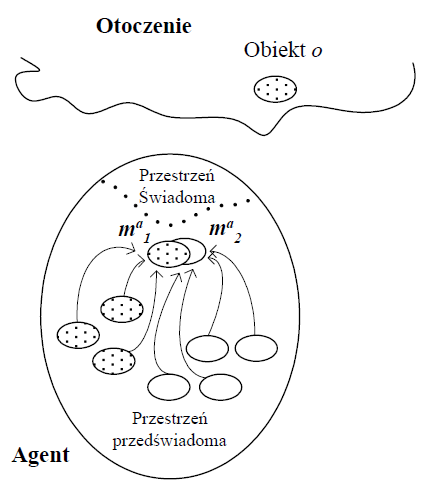
\includegraphics[width=.5\textwidth]{img/holon-modele-mentalne}
\end{figure}

Podstawą do ugruntowania przekonań agenta na temat cechy $ P $ w obiekcie $ o $ są wyrażenia $ p(o) $ i $ \neg p(o) $. Modele mentalne widoczne na rysunku \ref{rys:holon} rozumiane są jako struktury odsyłające do epizodów przechowywanych w prywatnej bazie, które reprezentują zebrane przez agenta doświadczenia o obecności ($ m^a{}_1 $) albo braku ($ m^a{}_2 $) cechy $ P $ w obiekcie $ o $. Doświadczenia te nazwano zbiorami gruntującymi. Liczność tych zbiorów definiuje siłę ugruntowania przekonań --- częstsze obserwacje skutkują silniejszymi przekonaniami agenta. 

Siła przekonań, wyrażona jako względna moc zbioru gruntującego ma bezpośredni wpływ na modalność zdania wyrażającego przekonanie agenta. Holon, oprócz kodowania sensu zdań modalnych, jest więc także bezpośrednią reprezentacją powierzchniową przekonań agenta.

Agent korzysta z holonów w sytuacjach, w których określenie stanu danej cechy w obiekcie rzeczywistym nie jest możliwe w oparciu o bieżący (najnowszy) epizod. Brak możliwości bezpośredniego stwierdzenia stanu cechy wypełniany jest przez agenta procesami gruntującymi, w wyniku których powstaje holon.

Opracowanie nowego modułu zarządzania bazą semantyczną holonów jest tematem tej pracy.





